\documentclass[12pt, openany]{scrbook}

\setkomafont{author}{\scshape}
\linespread{1}
\usepackage[margin=1in]{geometry} % 1 inch margins all around
\usepackage{graphicx} 
\usepackage{indentfirst}
\usepackage{enumitem}
\usepackage[font=small,labelfont=bf]{caption}
\RedeclareSectionCommand[beforeskip=0pt, afterskip=1cm]{chapter}

\title{What's Good Here?}
\subtitle{A new feature for Yelp to answer one of diner's top questions}
\date{June 2018}
\author{Josh Reid\thanks{University of Waterloo} \\ Email: jsreid13@gmail.com}

\begin{document}
\maketitle

\chapter{Introduction}

This submission comes from personal experience when dining at new restaurants,
trying to figure out what meals are good at this restaurant.
The pursuit of this information leads to scrolling through potentially
hundreds of reviews to find the ones that talk about the meal they
ordered, and then gauge whether or not they thought it was good.
This is very time consuming and usually results in the customer not
reading all of the reviews, when maybe further down there was a review
that mentioned a food was good that they would have liked even more.
This can result in a potentially disappointing dining experience that could 
have been improved if there had been a tool within Yelp that scanned
through all of the reviews and finding the reviews that talk about the meals at each
restaurant to tell the user which meals are good, and which ones to avoid.

In this report I propose a new feature for Yelp called \emph{What's Good Here?}
where users can now look within the page for restaurants to not just
find that average rating of that restaurant with reviews and photos, but also the average
ratings of all the different menu items that are mentioned within the reviews.
This will be in within the app just before the reviews section to provide users
a way to easily swipe through all the meals, similarly to the current keyword
detection within reviews.
When the user swipes through the meals they are shown the average rating for
each meal in brackets, and when that meal is pressed on then it retrieves the
reviews that talk about that meal.
A visual example of how this would look is shown in Figure 1.

\begin{center}
\noindent
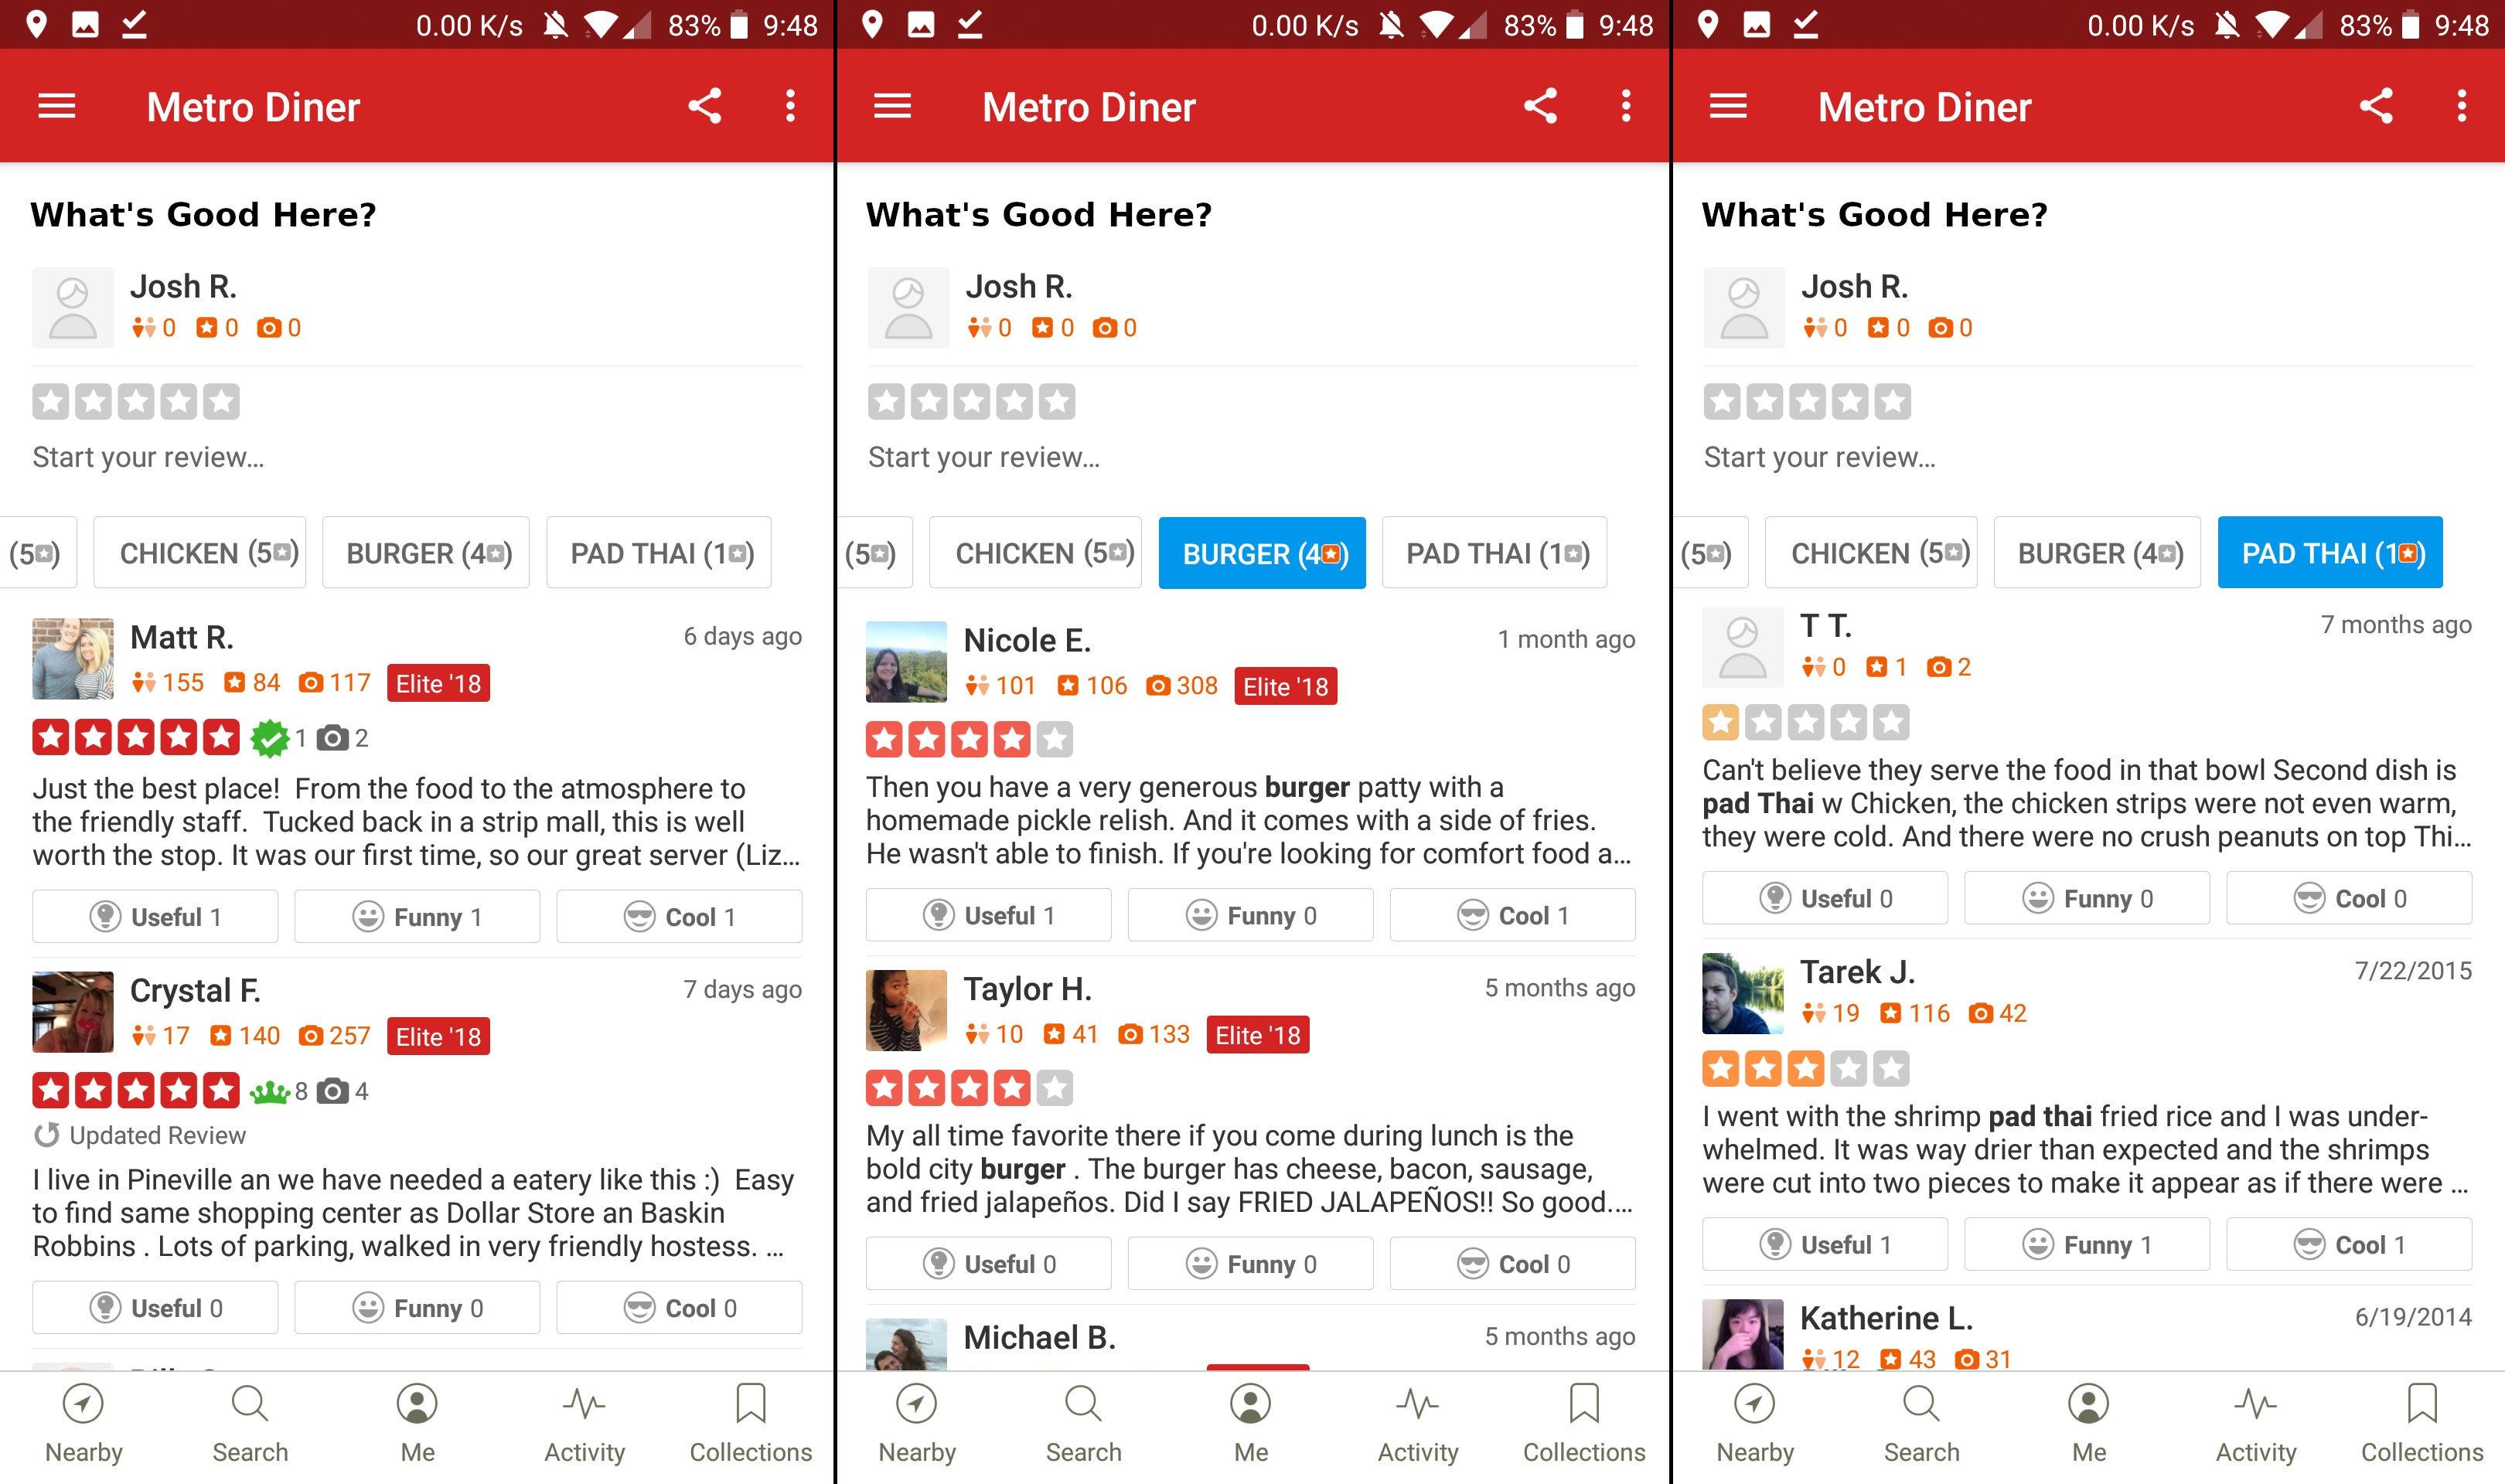
\includegraphics[width=\textwidth]{yelp_whats_good_here_combined.jpg}
\captionof{figure}{Layout of \emph{What's Good Here?} within the Yelp app showing
how meal names are listed in descending order of average star rating. When a meal
word is tapped then it brings up the reviews that mention that food.}
\end{center}

\chapter{Methods}

This entire project is written in Python and uses the provided SQL Yelp
database containing over 3 million reviews for 54618 different restaurants.
This section will go through the main parts of the code in detail here
to explain how \emph{What's Good Here?} works:

\section{Stemming}
First, the words in the reviews must be made consistent to allow for effective
detection and comparison of the reviews.
The possible options were to use a stemmer or lemmatizer.
Stemmers are tools that take words and remove any suffixes or prefixes to get a
root word. 
Lemmatizers do a similar job as stemmers, just that they are more intelligent and take into
account the word itself to see if there is a different root word based on
English grammar instead of just blindly chopping off suffixes and prefixes.
A good example of this is the word ``better''.
Where a stemmer would remove the suffix and leave you with ``bet'', a 
lemmatizer would know that better's root word is actually ``good'' and return that.
Lemmatizers are also beneficial because they return actual words, where stemmers
frequently return a root word that doesn't make sense.
For these reasons, a lemmatizer was used on the words in reviews to allow 
for consistent detection of words of interest.

\section{Building a Set of Valid Meals}
Next, a list is created that contains all of the names of meals to look for
within each review (technically its a set because this allows for faster 
searching and removes any duplicate words so they are not counted multiple times).
This list of words was scraped from a few different sources:
lists of different foods scraped off of a website\cite{vfg}, a list
of meal words from the Food101 food image recognition dataset and from
the a dataset built into the Natural Language ToolKit (NLTK) Python library.
This library include several datasets, including lists of words that are
semantically similar to each other called wordnets.
In this case the hyponym wordnet for ``food'' was used as this contains 
any word that falls under the category of food.
These words are then put into a list and any name that consists of
multiple words is stored as a tuple where each individual word is an element.
This is then converted to a set called \textbf{meal\_set}.

\section{Interacting with the SQL Database}
A connection is opened to the SQL database to begin sending
and retrieving information from it using the library pymysql.
The first step is to ensure that there is an index on the column
``business\_id'' within the ``review'' table otherwise the following
queries will take a long time.
Next, a list of the business\_ids that are restaurants is retrieved
that will be iterated through to extract the reviews for each business.
A business\_id is determined to be a restaurant by looking to see if it
has the category ``Restaurants'' within the table table ``category''.
This is used later for multiprocessing so that each process can be given
a chunk of business\_ids to work on to speed up the runtime of this script.
The business\_ids are used to find the reviews for that restaurant within 
the ``reviews'' table and are retrieved as a list.

\section{Analysing the Reviews}
Since analysing every word in all the reviews would take a long
time, most of the words that are likely not going to be a meal name
are stripped away.
This is achieved through the use of NLTK's Part Of Speech (POS)
tags which looks at each word in a review to determine what part of
speech that word is (verb, noun, adjective, pronoun, etc.).
This algorithm within NLTK also takes into account the context of words by looking at the
other words within the sentence to better determine the correct POS tag.
After the reviews are tagged, every word that is a noun or adjective
is saved to a list called \textbf{possible\_meal\_names}.
This is done because most meal names will consist of nouns that are sometimes
grouped with adjectives.

Every entry in \textbf{possible\_meal\_names} is then searched for within
the set of valid meals (\textbf{meal\_set}) and if found it is added to a separate list.
The score of that review is then appended to each meal name found.
Meal names for other reviews for that restaurant are also added to this
list with their respective score.
The review\_id is also appended to this list along with the score to keep
track of which review it came from so that the user interface not
only shows the average score for each meal is given but also the contents of the
review that mentioned it so the user can read the actual review to get
a more in depth description of the meal.
This is summarized below in Algorithm 1 together with multiword detection
discussed in the next section.

Once every review for a restaurant has been analysed the final list is
written back into the database under a new table called ``meal\_scores''.
The first column of this table is the ``restaurant\_id'', next is the name of the meal,
next is the average number of stars given by reviewers for that meal and the
final column are the individual review\_ids and the score they gave in JSON
syntax.
This is similar to what was done in the provided table ``attribute'' under
the column ``value'' so it is consistent with Yelp's database.

\section{Finding Meals with Multiword Names}
This works for finding meal words that consist of only a single word,
but there are many foods that are two or more words long.
This was handled by not only looking for each individual noun or adjective
that was found to see if it is within \textbf{meal\_set}, but to also see
if the next word is also a noun or adjective.
If it is, look for that word individually and for the combination of the two words.
This continues, adding more adjacent words as long as they're nouns or
adjectives until one is not found, then the combined word is cleared
until another noun or adjective is found.
This process is demonstrated in Algorithm 1.

\newpage
\vspace{12pt}
\hrule
\vspace{2pt}
\textbf{Algorithm 1} Finding Meal Names from a Corpus
\vspace{2pt}
\hrule
\vspace{2pt}
\textbf{Input:}\\A review, \emph{R};\\\textbf{meal\_set}\\
\textbf{Output:	meals\_with\_stars}
\begin{enumerate}[nosep]
  \item Split review \emph{R} into a list of words
  \item \emph{For} each word in the review
  \item Use NLTK \textbf{pos\_tag} to determine the word's POS tag
  \item \emph{If} the POS tag is noun (N) or adjective (J) 
  \item \hspace{12pt} Lemmatize that word
  \item \hspace{12pt} Append that word to a list of words \textbf{possible\_meal\_names}
	to later see if they're within \textbf{meal\_set}
  \item \hspace{12pt} \emph{If} the preceding word is not a noun or adjective,
	add this word to a string \textbf{multiword\_name} 
  \item \hspace{12pt} \emph{Else} append this word to the string \textbf{multiword\_name}
	and add this to the list \textbf{possible\_meal\_names} to see if this is a multiword meal name
  \item \emph{Else} clear \textbf{multiword\_name} as the adjacency of any nouns is now broken
  \item At the end of the review lemmatize each word within the list of
	the words \textbf{possible\_meal\_names}
  \item \emph{If} a word from \textbf{possible\_meal\_names} is found in
	\textbf{meal\_set} add it to the list \textbf{output}
  \item \textbf{return output}
\end{enumerate}
\vspace{8pt}
\hrule
\vspace{12pt}

This works well for finding words that are guaranteed to be meals based
on the words provided when building the \textbf{meal\_set}, however it misses out
on some meal names that are a combination of different meal words.
For example, ``chicken bacon club sandwich'' would be missed
because it wasn't specifically added to \textbf{meal\_set}, even though
each of those terms is present within \textbf{meal\_set} individually.
The alternative is to check every combination of \textbf{possible\_meal\_names}
within a review against each combination of individual words within the \textbf{meal\_set}.  
However, this method returned many incorrect results as meals like ``Pad Thai'' and 
``Polish sausage'' would return any review that mentioned Thai or Polish,
which for some restaurants would be many of the comments.
For this project it was decided to go with the safer approach to avoid
erroneous results that look bad from the users perspective
and use the first method without checking every combination of words.

\chapter{Results}

Comparing this to Yelp's current word detection within reviews on the mobile app
reveals that the word detection presented in this report is better at
detecting multiword meal names.
After checking several restaurants it was found to happen twice, which were
``All You Can Eat'' and ``Pad Thai''.
However even at the Vietnamese restaurant with the detected Pad Thai the Yelp
keyword detection only detected ``Curry'' as a keyword, even though
many of those reviews specified green or golden curry.
Yelp's keyword detection is better at pulling out general words
describing the restaurant though, such as ``Delivery'' and ``Wait''
which are also very useful to people looking for a place to eat.

\emph{What's Good Here?} will be very useful to the user by providing an 
average score for each meal to quickly give the user an overview of all
the meals talked about at the restaurant.
This will help guide their decision to picking a meal that will give them
and enjoyable experience at that restaurant thanks to Yelp.
This will then increase the chance that they will come back to that restaurant
and will make Yelp their first choice for an app when looking up places to go eat.

Running this code on the entire dataset revealed that 66\% of reviews
contained at least one entry in \textbf{possible\_meal\_names}.
This shows that a large number of restaurant reviews mention food
served at each restaurant, providing a sufficiently large dataset
of meal reviews that can be used to provide accurate
meal recommendations to their users.

In order to determine the recall of this algorithm all the reviews for
one restaurant with 140 reviews were looked at manually to find all meal names.
Then this was compared to the results returned from this algorithm to see how
many of the meal words were found to determine the recall of this algorithm.
After this analysis it was determined that the recall of this algorithm
was 69\%, while this is good it definitely will need to be improved by further
expanding the \textbf{meal\_set} with more valid meal names.
Since false positives are almost impossible with this algorithm due to the
use of the handmade \textbf{meal\_set} to determine the validity of words being meals,
the precision is near 100\%.

\chapter{Conclusion}

With the determined accuracy and prevalence of meal names found within reviews after
only a few weeks of work it is my belief and hopefully yours now too that there
is great potential for a feature like this to be used across all restaurant pages
on Yelp.
With the additional resources available at Yelp I believe \emph{What's Good Here?}
could be implemented within your apps quickly, building on top of your
currently existing keyword finding feature within the reviews on Yelp.
This will provide users a unique tool for when they arrive at restaurants
unsure of what to eat that only Yelp provides currently.

If a feature like this was to be implemented within Yelp there are a
couple of additional features that I think should be added with more
time and resources to work on this to make it truly amazing.

\section{Future Work}
\begin{itemize}
  \item Currently only meal words are extracted from English reviews, but with Yelp
		being popular across the globe this is something that would need to be
		expanded to support more languages. This can be solved by expanding the
		set of meal words that this script looks for within reviews to include
		multiple languages.
		For example, support for Chinese could be implemented through a meal
		detection algorithm similar to the one proposed by Xu and Qiu\cite{xu2015}.
  \item There is the potential of returning reviews that in fact didn't like that meal
		but had a high score if the user gave a high score for other reasons.
		This could be solved through sentiment analysis of the actual sentence that
		mentioned the name of the meal.
  \item Currently within this script there is no way to determine the quality of
		a review, this would be beneficial so that when a user is looking through
		reviews for each meal they are presented high quality reviews first to
		speed up their decision making.
  \item Add a feature such that Yelp provides suggestions to users to mention
		detected meal names for that restaurants to improve the detection
		and increase the number of reviews that mention meals.
  \item Add a section for best foods at that restaurant, determined as ones that have a
		consistently high score amongst reviewers after a minimum of several reviews.
  \item A foods to avoid section would also be useful for the users and that restaurant owner
		to help them in determining which areas need improvement in their restaurant.
\end{itemize}


\noindent Thank you for considering this project, and I look forward to hearing back from
you with any feedback on this report.

\begin{thebibliography}{9}

\bibitem{vfg}
  \emph{Vegetables Fruit Grains}.
  http://vegetablesfruitsgrains.com
  2018.
\bibitem{xu2015}
  Ge Xu, Likun Qiu,
  \emph{Extracting Food Names from Food Reviews}.
  IEEE/WIC/ACM International Conference on Web Intelligence and Intelligent Agent Technology
  2015.

\end{thebibliography}

\end{document}

